\documentclass[10pt,journal,compsoc]{IEEEtran}

% *** CITATION PACKAGES ***
%
\ifCLASSOPTIONcompsoc
  % IEEE Computer Society needs nocompress option
  % requires cite.sty v4.0 or later (November 2003)
  \usepackage[nocompress]{cite}
\else
  % normal IEEE
  \usepackage{cite}
\fi

\usepackage{graphicx}
\graphicspath{ {Images/} }
\usepackage{amssymb}
\usepackage{listings}
\usepackage{color}
\usepackage[table,xcdraw]{xcolor}

\definecolor{dkgreen}{rgb}{0,0.6,0}
\definecolor{gray}{rgb}{0.5,0.5,0.5}
\definecolor{mauve}{rgb}{0.58,0,0.82}

\lstset{frame=tb,
  language=Python,
  aboveskip=3mm,
  belowskip=3mm,
  showstringspaces=false,
  columns=flexible,
  basicstyle={\small\ttfamily},
  numbers=none,
  numberstyle=\tiny\color{gray},
  keywordstyle=\color{blue},
  commentstyle=\color{dkgreen},
  stringstyle=\color{mauve},
  breaklines=true,
  breakatwhitespace=true,
  tabsize=3,
  morekeywords={if, in, or, then, enter, into, end, command, delete, from, not, create},
  xleftmargin=\dimexpr 1em+3pt\relax,
  linewidth=\dimexpr \linewidth-3pt\relax
}

\lstnewenvironment{itemlisting}[1][]
 {%
  \mbox{}
  \vspace*{-\baselineskip}
  \lstset{
    xleftmargin=\leftmargin,
    linewidth=\linewidth,
    #1
  }%
 }
 {}
 
% correct bad hyphenation here
\hyphenation{op-tical net-works semi-conduc-tor}

\renewcommand{\arraystretch}{1.5}

\begin{document}

\title{CS 6600 Project Report: Unmanned Aircraft System}

\author{Matthew Whitesides and Bruce M. McMillin \\
Department of Computer Science \\
Missouri University of Science and Technology, Rolla, MO 65409-0350} 

% The paper headers
\markboth{Missouri S\&T COMP\_SCI 6600: Formal Methods in CmpSec, Fall~2021}%
{Shell \MakeLowercase{\textit{et al.}}: Bare Demo of IEEEtran.cls for Computer Society Journals}
 
% The paper abstract
\IEEEtitleabstractindextext{%
\begin{abstract}
The abstract goes here.
\end{abstract}}

% make the title area
\maketitle

\IEEEpeerreviewmaketitle

%-------------------------------------------------------------------------

\section{Infrastructure}

\subsection{Infrastructure Description}

\IEEEPARstart{I}{n} its simplest form, an unmanned aircraft system (UAS), is an aircraft system that operates without an onboard pilot. 
UAS are either controlled remotely through some form of wireless radio communication, semi-autonomously in conjunction with a remote pilot, or fully autonomously using some form of computational intelligence as navigation. 
These intelligent crewless vehicles have many potential uses in the defense sector, including surveillance, strategic mission execution, aerial sustainability support, and training systems, to name a few. 
These aircraft fall under the umbrella of cyber-physical systems (CPS), merging the intelligent navigation processes, system health monitoring, and communication with the physical mobile aerial vehicle.

We will design a proposed infrastructure security policy for the Boeing MQ-25 unmanned aircraft system, but it will also apply to similar mission support drones. 
The MQ-25 is an unmanned aircraft system designed for the U.S. Navy, and it provides autonomous refueling capability for the Boeing F/A-18 Super Hornet, Boeing EA-18G Growler, and Lockheed Martin F-35C fighters.
This capability extends the combat range of the supported aircraft, seamlessly and semi-anonymously navigating to the plane, refueling, and returning to base. 
MQ-25 is the first unmanned aircraft to support aerial refueling another aircraft and is currently in the flight test phase of development [1], making it the perfect system to analyze security impacts for current and future unmanned aircraft systems. 

\subsubsection{Infrastructure Security Policy}

\begin{table}[]
  \caption{Description of rights over objects in the UAS.}
  \begin{tabular}{ll}
  \hline
  \textbf{Right}       & \textbf{Description}                               \\ 
  \hline
  \textit{Owns (O)}    & The owner of the given object.                     \\
  \textit{Read (R)}    & Can observe the given object.                      \\
  \textit{Write (W)}   & Can modify the given object.                       \\
  \textit{Execute (E)} & Can execute the functionality of the given object. \\
  \textit{Grant (G)}   & Can grant a given right to another subject.        \\
  \textit{Control (C)} & Can control a given system object.                 \\
  \textit{Delete (C)}  & Can delete a given object or right.                 \\
  \textit{Create (C)}  & Can create a new subject or object.                 \\
  \hline
  \end{tabular}
\end{table}

\begin{table*}[]
  \caption{Description of actor subject roles during a UAS refueling mission.}
  \begin{tabular}{ll}
  \hline
  \textbf{Subject}                           & \textbf{Description}                                                                                       \\ 
  \hline
  \textit{Pilot Commander (PC)}                  & The primary remote pilot of the UAS during the mission.                                                    \\
  \textit{Instructor Pilot (IP)}                 & Assists the Pilot Commander and can pilot the UAS if given permission from the PC or MC.                   \\
  \textit{Maintenance Crew (MC)}                 & Handles work orders created by the PC, IP, or FDA, responsible for the maintenance of the UAS.             \\
  \textit{Flight Data Admin (FDA)}               & Handles and analyses all mission flight data.                                                              \\
  \textit{External Contractor (Bad Actor) (EC)}  & Has a similar job to the MC however only has read rights to the FED.                                       \\
  \hline
  \end{tabular}
\end{table*}

\begin{table*}[]
  \centering
  \caption{Initial UAS Refueling Mission Access Control Matrix}
  \label{tab:initial-acm}
  \resizebox{\textwidth}{!}{
    \begin{tabular}{l|llllllllll}
      \hline
      \textbf{}                                        & \textit{PC}   & \textit{IP}   & \textit{MC}   & \textit{FDA}  & \textit{BA}   & \textbf{ANC}  & \textbf{RO}   & \textbf{FED}  & \textbf{RTD}  & \textbf{FRS}  \\
      \hline
      \textit{Pilot Commander (PC)}                    & O,R,W         & R,W           & R,W           & R,W           & R,W           & O,R,W,E,G,C   & O,R,W,E,G,C   & R,W,E,G,C     & R,W,E,G,C     & R,W,E,G,C     \\
      \textit{Instructor Pilot (IP)}                   & R             & O,R,W         & $\varnothing$ & $\varnothing$ & $\varnothing$ & R,W,E,C       & R,W,E,C       & R,E           & R,E           & R,E           \\
      \textit{Maintenance Crew (MC)}                   & $\varnothing$ & $\varnothing$ & O,R,W         & R             & R             & $\varnothing$ & $\varnothing$ & R,E           & R,E           & R,E           \\
      \textit{Flight Data Admin (FDA)}                 & $\varnothing$ & $\varnothing$ & R             & O,R,W         & O,R,W         & $\varnothing$ & $\varnothing$ & O,R,W,E,G,C   & O,R,W,E,G,C   & O,R,W,E,G,C   \\
      \textit{Maintenance Contractor (Bad Actor) (BA)} & $\varnothing$ & $\varnothing$ & $\varnothing$ & $\varnothing$ & O,R,W         & $\varnothing$ & $\varnothing$ & $\varnothing$ & R             & $\varnothing$ \\
      \textbf{Autonomous Navigation Control (ANC)}     & $\varnothing$ & $\varnothing$ & $\varnothing$ & $\varnothing$ & $\varnothing$ & R,W,E,C       & R             & R             & R             & $\varnothing$ \\
      \textbf{Refueling Operation (RO)}                & $\varnothing$ & $\varnothing$ & $\varnothing$ & $\varnothing$ & $\varnothing$ & $\varnothing$ & R,W,E,C       & R             & R             & $\varnothing$ \\
      \textbf{Flight Engine Data (FED)}                & $\varnothing$ & $\varnothing$ & $\varnothing$ & $\varnothing$ & $\varnothing$ & $\varnothing$ & $\varnothing$ & R,W,E,C       & $\varnothing$ & $\varnothing$ \\
      \textbf{Refueling Tank Data (RTD)}               & $\varnothing$ & $\varnothing$ & $\varnothing$ & $\varnothing$ & $\varnothing$ & $\varnothing$ & $\varnothing$ & $\varnothing$ & R,W,E,C       & $\varnothing$ \\
      \textbf{Flight Record System (FRS)}              & $\varnothing$ & $\varnothing$ & $\varnothing$ & $\varnothing$ & $\varnothing$ & $\varnothing$ & $\varnothing$ & $\varnothing$ & $\varnothing$ & R,W,E,C      
    \end{tabular}}
  \end{table*}

  \begin{table*}[]
    \centering
    \caption{ACM After Create Flight Record}
    \label{tab:table-after-create-flight-record}
    \resizebox{\textwidth}{!}{
    \begin{tabular}{l|lllllllllll}
      \hline
      \textbf{}    & \textit{PC}                          & \textit{IP}                          & \textit{MC}                          & \textit{FDA}                         & \textit{BA}                          & \textbf{ANC}                         & \textbf{RO}                          & \textbf{FED}                         & \textbf{RTD}                         & \textbf{FRS}                         & {\color[HTML]{009901} \textbf{FR}}   \\
      \hline
      \textit{PC}  & O,R,W                                & R,W                                  & R,W                                  & R,W                                  & R,W                                  & O,R,W,E,G,C                          & O,R,W,E,G,C                          & R,W,E,G,C                            & R,W,E,G,C                            & R,W,E,G,C                            & {\color[HTML]{009901} R,W,E,G,C}     \\
      \textit{IP}  & R                                    & O,R,W                                & $\varnothing$                        & $\varnothing$                        & $\varnothing$                        & R,W,E,C                              & R,W,E,C                              & R,E                                  & R,E                                  & R,E                                  & {\color[HTML]{009901} R,E}           \\
      \textit{MC}  & $\varnothing$                        & $\varnothing$                        & O,R,W                                & R                                    & R                                    & $\varnothing$                        & $\varnothing$                        & R,E                                  & R,E                                  & R,E                                  & {\color[HTML]{009901} R,E}           \\
      \textit{FDA} & $\varnothing$                        & $\varnothing$                        & R                                    & O,R,W                                & O,R,W                                & $\varnothing$                        & $\varnothing$                        & O,R,W,E,G,C                          & O,R,W,E,G,C                          & O,R,W,E,G,C                          & {\color[HTML]{009901} O,R,W,E,G,C}   \\
      \textit{BA}  & $\varnothing$                        & $\varnothing$                        & $\varnothing$                        & $\varnothing$                        & O,R,W                                & $\varnothing$                        & $\varnothing$                        & $\varnothing$                        & R                                    & {\color[HTML]{CB0000} E,W}             & {\color[HTML]{009901} $\varnothing$} \\
      \textbf{ANC} & $\varnothing$                        & $\varnothing$                        & $\varnothing$                        & $\varnothing$                        & $\varnothing$                        & R,W,E,C                              & R                                    & R                                    & R                                    & $\varnothing$                        & {\color[HTML]{009901} $\varnothing$} \\
      \textbf{RO}  & $\varnothing$                        & $\varnothing$                        & $\varnothing$                        & $\varnothing$                        & $\varnothing$                        & $\varnothing$                        & R,W,E,C                              & R                                    & R                                    & $\varnothing$                        & {\color[HTML]{009901} $\varnothing$} \\
      \textbf{FED} & $\varnothing$                        & $\varnothing$                        & $\varnothing$                        & $\varnothing$                        & $\varnothing$                        & $\varnothing$                        & $\varnothing$                        & R,W,E,C                              & $\varnothing$                        & $\varnothing$                        & {\color[HTML]{009901} $\varnothing$} \\
      \textbf{RTD} & $\varnothing$                        & $\varnothing$                        & $\varnothing$                        & $\varnothing$                        & $\varnothing$                        & $\varnothing$                        & $\varnothing$                        & $\varnothing$                        & R,W,E,C                              & $\varnothing$                        & {\color[HTML]{009901} $\varnothing$} \\
      \textbf{FRS} & $\varnothing$                        & $\varnothing$                        & $\varnothing$                        & $\varnothing$                        & $\varnothing$                        & $\varnothing$                        & $\varnothing$                        & $\varnothing$                        & $\varnothing$                        & R,W,E,C                              & {\color[HTML]{009901} $\varnothing$} \\
      {\color[HTML]{009901} \textit{\textbf{FR}}} & {\color[HTML]{009901} $\varnothing$} & {\color[HTML]{009901} $\varnothing$} & {\color[HTML]{009901} $\varnothing$} & {\color[HTML]{009901} $\varnothing$} & {\color[HTML]{009901} $\varnothing$} & {\color[HTML]{009901} $\varnothing$} & {\color[HTML]{009901} $\varnothing$} & {\color[HTML]{009901} $\varnothing$} & {\color[HTML]{009901} $\varnothing$} & {\color[HTML]{009901} $\varnothing$} & {\color[HTML]{009901} R,W,E,C}      
    \end{tabular}}
  \end{table*}

  Our infrastructure security policy breaks down the various actions a system user can perform using the following terms. 

  \begin{itemize}
    \item \textit{Subject}: Any entity that contains the proper rights can request the UAS perform operations, access objects, or grant rights to another subject.
    \item \textit{Object}: An entity that is part of the UAS functionality or data that does not have control over another entity. 
    \item \textit{Rights}: A property assigned to a subject that defines its right to access an object or grant permissions to another subject.
  \end{itemize}
  
  Table 1 describes the rights and their associated functionality. Table 2 breaks down the subject roles involved in operating the UAS during a refueling mission. Table 3 contains the access control matrix (ACM) showing each Subject's rights over the objects.
  
  \subsection{HRU}
  
  The following shows the basic HRU commands related to our UAS mission.
  A fundamental UAS refueling mission follows these basic steps. 

  \begin{enumerate}
    \item UAS is verified flight-ready by the MC.
    \item The PC plans the mission.
    \item The PC and IP execute the mission.
    \item During the flight, the PC and IP execute the ANC and RO as needed.
    \item After the refueling operation, the UAS returns to base, and the flight is debriefed. 
    \item PC, IP, or MC download the flight data from the UAS flight recorder. 
    \item A flight record (FR) is created that contains flight tracking information, engine usage data, and various UAS health status.
    \item This flight record is uploaded by the PC, IP, MC, or BA to the record-keeping system. 
    \item Mission is completed. 
  \end{enumerate}
  
  With this in mind, we have the following basic HRU commands available for post-flight maintenance (steps 5 - 9). We will then show how improper use of these commands can lead to a rights leakage with our external contractor standing in as our ``bad actor'' gaining a leak of Integrity and confidentiality rights beyond our initial ACM. 

  The first command is a generic \textit{Grant r Rights} that allows a subject to grant any right they have over a subject/object to another subject/object.

\begin{lstlisting}
command grant_r_right(r, o, p, q)
  if grant in A[p, o] and r in A[p, o]
  then
    enter r into A[q, o];
end
\end{lstlisting}
    
  Next we have command \textit{Make Owner} allowing a subject \textit{p} to make another subject \textit{q} the owner of a object \textit{o} they currently have owner rights over. 

\begin{lstlisting}
command make_owner(p, q, o)
  if owns in A[p, o]
  then
    enter owns into A[q, o];
end
\end{lstlisting}
  
  When the \textit{PC} and \textit{IP} return from a flight they or a \textit{MC} will read the flight data and create a new object \textbf{Flight Record (FR)} holding the flight data, available to subjects who have \textbf{FED} access. 
  After running this command, our ACM would transition to a new state similar to table 4, representing the subjects and objects involved in the create flight record procedure. 
  This command will also give rights to the FRS to control the flight record data once uploaded.
  
\begin{lstlisting}
command create_flight_record(p)
  if create in A[p, FED]
  then
    create object FR;
    enter own into A[p, FR];
    enter delete into A[p, FR];
    enter read into A[p, FR];
    enter grant into A[p, FR];
end
\end{lstlisting}

After creating a flight record which may be done by a PC, IP, or MC, they may choose to give the task of processing and uploading the flight record to an external maintenance contractor and execute the following command to provide them with access to the record. 
In the command \textit{Grant Flight Record Access}, \textit{p} is the subject granting the right to subject \textit{q}, for the \textit{fr} flight record.

\begin{lstlisting}
command grant_flight_record_access(p, q, fr)
if own in A[p, fr]
then
  enter read into A[q, FR];
  enter write into A[q, FR];
  enter execute into A[q, FR];
end
\end{lstlisting}  

Finally, the flight record needs to be uploaded to our flight record system using the following \textit{Upload Flight Record} command with \textit{p} being the subject executing the command and \textit{fr} being flight record to upload.

\begin{lstlisting}
command upload_flight_record(p, fr)
if own in A[p, fr] and read in A[p, FRS]
then
  enter read into A[FRS, FR];
  enter write into A[FRS, FR];
  enter execute into A[FRS, FR];
  enter control into A[FRS, FR];
end
\end{lstlisting}

Similar to \textit{Create Flight Record} a subject may need to delete or update a flight record from the system. 

\begin{lstlisting}
command delete_flight_record_from_system(p, FR)
if delete in A[p, FR]
then
  delete read from A[FRS, FR];
  delete write from A[FRS, FR];
  delete execute from A[FRS, FR];
  delete control from A[FRS, FR];
end
\end{lstlisting}

If any modifications need to be made to the FRS, the following command begins an update transaction and ends one for a given subject and flight record. 

\begin{lstlisting}
command begin_update_frs(p, FR)
if write in A[p, FR]
  then
    enter write into A[p, FRS];
end
\end{lstlisting}

\begin{lstlisting}
  command end_update_frs(p, FR)
  if write in A[p, FR]
    then
      delete write from A[p, FRS];
  end
\end{lstlisting}

\subsection{Rights Leakages}
  
\subsubsection{Confidentiality}

  For our example of a confidentiality attack, we simulate a scenario where our \textit{External Contractor} is a bad actor seeking leaked rights beyond the initial ACM utilizing the following HRU commands available for the UAS.

  The following sequence of commands is typical among a mission debriefing process. 

\begin{lstlisting}
create_flight_record(Maintenance Crew (MC));
grant_flight_record_access(Maintenance Crew, Maintenance Contractor (BA), Flight Record (FR));
upload_flight_record(Maintenance Contractor (BA), Flight Record (FR));
\end{lstlisting}  

  However, when running \textit{Update Flight Record System}, the BA will find they do not have ``own'' rights over the record, which is required so that they will go back to the original MC and as to grant them execute privileges to the FRS system. 
  The MC will execute the commands to make BA have permission to upload the FR. 

\begin{lstlisting}
make_owner(MC, BA, FR);
command grant_r_right(execute, FRS, MC, BA);
\end{lstlisting}

  This command, unfortunately, will lead to a leak as the contractor (BA) now has the execute privileges over the FRS, which they did not initially and is not intended and can lead to other flight records confidential information being exposed to the BA. 
  Table 4 shows the leaked rights in red. 

\subsubsection{Integrity}

  In an attempt at an integrity leak, our BA may seek out modifying existing data and, to get permission to do so, may attempt the following sequence. 

\begin{lstlisting}
create_flight_record(Maintenance Crew (MC));
grant_flight_record_access(Maintenance Crew, Maintenance Contractor (BA), Flight Record (FR));
upload_flight_record(Maintenance Contractor (BA), Flight Record (FR));
make_owner(MC, BA, FR);
update_flight_record_system(BA, FR);
\end{lstlisting}  

  However, upon reviewing the FR, the MC notices an issue in the data and wants the BA to update the flight record system. 
  Unfortunately, \textit{Update Flight Record System} checks only for rights to the given flight record and not the initial systems, therefore, giving the BA \textit{write} access to the FRS system, which could lead them modifying the FRS data ruining its integrity.
  Table 4 shows the result of executing the confidentiality and integrity leaks. 

\section{Survey}

\subsection{Take-Grant}

  Next, we take a look at the Take-Grant (TG) model interpretation of our rights leakages. 
  This models our HRU example in terms of a TG model where the \textit{Flight Record} created object has \textit{read, write} rights over the \textit{Flight Record System} that our \textbf{Maintenance Contractor (BA)} can utilize to gain \textit{read, write} access to the \textit{Flight Engine Data}.

  Our bad actor could achieve this leaked through the following TG commands. 

  \begin{enumerate}
    \item \textbf{BA} creates object \textbf{FR}.
    \item \textbf{MC} grants (\textit{t} to \textbf{FR}) to \textbf{BA}.
    \item \textbf{BA} takes (\textit{r,w} to \textbf{FRS}) from \textbf{FR}.
    \item \textbf{BA} takes (\textit{r,w} to \textbf{FED}) from \textbf{FRS}.
  \end{enumerate}

  Figure 1 shows the initial state of rights among actors and objects in the \textbf{FRS} system.

  \begin{figure}[t]
    \caption{Initial Iteration T-G Model Graph} 
    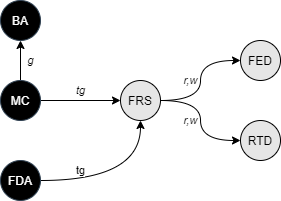
\includegraphics[scale=0.7]{TGModel1.png}
  \end{figure}

  Figure 2 shows the rights after the \textbf{MC} creates a new \textbf{FR} object. 

  \begin{figure}[t]
    \caption{Iteration 2 T-G Model Graph} 
    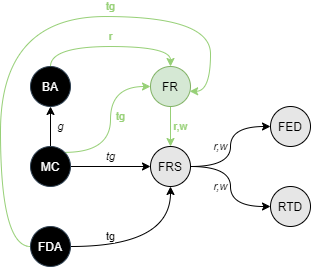
\includegraphics[scale=0.7]{TGModel2.png}
  \end{figure}

  Finally figure 3 shows how after the \textbf{BA} tricks the \textbf{MC} into giving them \textit{t} rights over \textbf{FR} they can exploit the system to take our laked rights to \textbf{FED} through the \textbf{FRS}.

  \begin{figure}[t]
    \caption{Final Iteration T-G Model Graph} 
    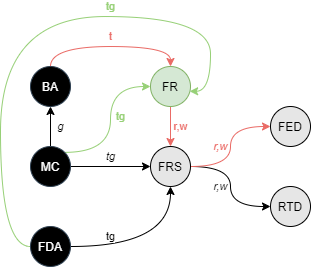
\includegraphics[scale=0.7]{TGModel3.png}
  \end{figure}


% \subsection{BLP}
% text
% \subsection{Biba}
% text
% \subsection{Noninference/Noninterference/ NonDeducibility}
% text
% \section{Specific Models and Rights Leakages}
% \subsection{HRU}
% text
% \subsection{T-G}
% text
% \subsection{BLP}
% text
% \subsection{Biba}
% text
% \subsection{Noninference}
% text
% \subsection{Noninterference}
% text
% \subsection{NonDeducibility}
% text
% \subsection{MSDND}
% text

% \section{Specific Models and Rights Leakages}
% \subsection{HRU}
% text
% \subsection{T-G}
% text
% \subsection{BLP}
% text
% \subsection{Biba}
% text
% \subsection{Noninference}
% text
% \subsection{Noninterference}
% text
% \subsection{NonDeducibility}
% text
% \subsection{MSDND}
% text

% \begin{figure}[h]
%    \caption{Example of caption.}
% \end{figure}

% \section{Conclusions}

% Provide a summative conclusion on the modeling of your infrastructure.

% Can use something like this to put references on a page
% by themselves when using endfloat and the captionsoff option.
\ifCLASSOPTIONcaptionsoff
  \newpage
\fi

\begin{thebibliography}{1}

\bibitem{IEEEhowto:kopka}
A.~Erwin, and J.~Gibson, Navy, Boeing Make Aviation History with MQ-25 Becoming the First Unmanned Aircraft to Refuel Another Aircraft, Accessed on: Sept. 1, 2021. [Online]. Available: https://www.boeing.com/defense/mq25/ 

\end{thebibliography}

% biography section
\begin{IEEEbiographynophoto}{Matthew Whitesides}
  Master's Student at Missouri University of Science and Technology.
\end{IEEEbiographynophoto}

% that's all folks
\end{document}


